\chapter[AGES II --- Pró-Mata]{AGES II --- \enquote{Pró-Mata}}

\section{Introdução}

O Centro de Pesquisas e Proteção da Natureza (CPPN) Pró-Mata desempenha
um papel essencial na preservação ambiental e também na promoção de
atividades acadêmicas, turísticas e culturais. Para atender melhor esse
público diverso, surgiu a necessidade de criar uma plataforma digital
que centralize e facilite o acesso aos serviços oferecidos pelo centro.

A iniciativa busca modernizar e tornar mais acessíveis processos que
antes eram manuais ou fragmentados, como reservas de hospedagem,
agendamento de atividades e organização de eventos. Com a plataforma,
espera-se proporcionar mais praticidade e transparência aos visitantes,
ao mesmo tempo em que se fortalece a gestão interna e se melhora a
experiência de todos que têm contato com o Pró-Mata --- sejam
estudantes, pesquisadores, turistas ou instituições parceiras.

Mais do que uma solução tecnológica, este projeto representa um passo
importante para aproximar o centro de sua comunidade, ampliando seu
alcance e reforçando sua missão de unir conservação, educação e turismo
sustentável.

\section{Desenvolvimento do Projeto}

\textbf{Stakeholder do Projeto:}

\begin{itemize}
\item
  Prof. Augusto Mussi Alvim
\end{itemize}

\textbf{Período de Execução}: Segundo semestre de 2025.

A Figura~\ref{fig:equipe-promata} apresenta os integrantes que participaram do
projeto Pró-Mata.

\begin{figure}[H]
  \centering
  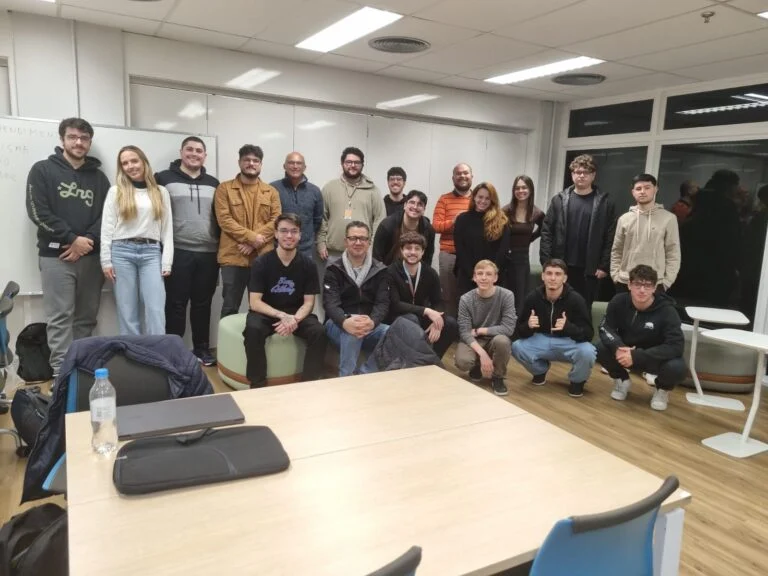
\includegraphics[width=\textwidth]{imagens/ProMata/equipe-promata.png}
  \caption{Equipe do projeto Pró-Mata}
  \label{fig:equipe-promata}
  \fonte{Acervo pessoal.}
\end{figure}

\begin{enumerate}
\def\labelenumi{\arabic{enumi}.}
\item
  \textbf{Repositório do código Fonte do Projeto}
\end{enumerate}

O código-fonte e a documentação do projeto estão disponíveis na
\href{https://tools.ages.pucrs.br/pro-mata}{wiki do Pró-Mata}.

O código fonte está hospedado no GitLab, onde todo o desenvolvimento
colaborativo é gerenciado.

\begin{enumerate}
\def\labelenumi{\arabic{enumi}.}
\setcounter{enumi}{1}
\item
  \textbf{Banco de Dados utilizado}
\end{enumerate}

A documentação do banco de dados está disponível na
\href{https://tools.ages.pucrs.br/pro-mata/wiki/-/wikis/Banco\%20de\%20Dados}{wiki do Pró-Mata}.

\begin{quote}
Diagrama das tabelas do banco de dados.

\textbf{Desenvolvimento}: Um contêiner PostgreSQL executado localmente. O Prisma
ORM gerencia as migrações automaticamente.

\textbf{Produção}: PostgreSQL com replicação master-slave, backups
automáticos criptografados, e monitoramento futuro com Grafana e
PostgreSQL exporter.
\end{quote}

\begin{enumerate}
\def\labelenumi{\arabic{enumi}.}
\setcounter{enumi}{2}
\item
  \textbf{Arquitetura utilizada}
\end{enumerate}

Os detalhes arquiteturais estão disponíveis na
\href{https://tools.ages.pucrs.br/pro-mata/wiki/-/wikis/Arquitetura}{wiki do Pró-Mata}.

Baseando-se no que foi planejado para o nosso banco de dados,
levantamento dos requisitos e o entendimento geral do time sobre o
projeto a ser desenvolvido, optamos por uma arquitetura de
Cliente-Servidor, onde há uma separação entre o frontend e backend.

\begin{enumerate}
\def\labelenumi{\arabic{enumi}.}
\setcounter{enumi}{3}
\item
  \textbf{Protótipos das telas desenvolvidas}
\end{enumerate}

Os protótipos das interfaces estão disponíveis na
\href{https://tools.ages.pucrs.br/pro-mata/wiki/-/wikis/Design}{wiki do Pró-Mata}.

Os mockups do projeto foram feitos no Figma, exibindo o design e fluxo
das interfaces.

\begin{enumerate}
\def\labelenumi{\arabic{enumi}.}
\setcounter{enumi}{4}
\item
  \textbf{Tecnologias Utilizadas}
\end{enumerate}

\begin{quote}
As decisões técnicas detalhadas estão disponíveis na
\href{https://tools.ages.pucrs.br/pro-mata/wiki/-/wikis/Arquitetura}{wiki do Pró-Mata}.

\textbf{React 19}: Construção de interfaces declarativas com componentes
reutilizáveis \cite{react}.

\textbf{TypeScript:} Tipagem estática (configuração em \texttt{tsconfig.json},
moduleResolution: "bundler", baseUrl, paths @/*).

\textbf{Vite 6} --- Servidor de desenvolvimento e \textit{build} otimizados
\cite{vite}; uso do plugin \texttt{@tanstack/router-plugin} para divisão
automática de código e geração de rotas.

\textbf{Tailwind CSS (v4)} --- Utilitários CSS e tokens de tema para as
variações claro/escuro \cite{tailwind}.

\textbf{TanStack Router} --- Roteamento baseado em arquivos, com guardas,
divisão de código e ferramentas de desenvolvimento \cite{tanstack-router}.

\textbf{TanStack Query} --- Cache e invalidação de dados; QueryClient
injetado no contexto do Router.

\textbf{shadcn/ui + Radix UI} --- Componentes acessíveis (dialog,
popover, select, table, sheet, etc.) com variantes (CVA).

\textbf{Zod + React Hook Form} --- Esquemas de validação tipados e
formulários controlados.

\textbf{Zustand} --- Estado leve e local (stores de UI e filtros).

\textbf{Axios} --- Cliente HTTP com \textbf{interceptor} de autenticação
(Bearer).

\textbf{ESLint/Prettier} --- Lint e formatação padronizada.

\textbf{Vitest} --- Testes unitários com run, watch e UI.

\textbf{Node.js / npm} --- Toolchain e scripts de desenvolvimento.
\end{quote}

\section{Atividades desempenhadas pelo aluno no projeto}

\subsection{Sprint 0}

A Sprint 0 foi dedicada a alinhar a visão do produto com protótipos
navegáveis no Figma e a colocar no ar os primeiros componentes do
frontend, organizando o fluxo de telas e preparando a base visual para
as próximas sprints.

\textbf{Atividades Desempenhadas:}

\begin{itemize}
\item
  Desenvolvimento no Figma: ajustes de mockups, criação de cards
  compactos, animações no Prototype e botão de idioma.
\item
  Definição do \textbf{System Flow} (user flow/screen flow) para
  orientar navegação e decisões de UI.
\item
  Implementação do \textbf{CardStatus} (enum de estados, ícones SVG,
  fallback para status desconhecido e estilos com Tailwind).
\item
  Desenvolvimento do \textbf{CardsInfoOnHover} (branch \#44): estrutura
  HTML, estilos com Tailwind, lógica de hover com useState, integração
  de imagens mock, posicionamento na Home; revisão de tipagem, ajustes
  com TanStack Router e \textbf{PR} entregue.
\item
  Ambientação/estudo do stack do frontend (React, TypeScript, Tailwind,
  TanStack Router, Zustand, React Hook Form + Zod, JWT) e ajustes de
  ambiente (VS Code, PostCSS, ícones).
\end{itemize}

\textbf{Ferramentas Utilizadas:}

\begin{itemize}
\item
  \textbf{Figma} (mockups e Prototype)
\item
  \textbf{React} + \textbf{TypeScript}
\item
  \textbf{Tailwind CSS}
\item
  \textbf{TanStack Router}
\item
  \textbf{Zustand}
\item
  \textbf{React Hook Form} + \textbf{Zod}
\item
  \textbf{Git/GitHub}, \textbf{VS Code}, PostCSS, SVGs
\end{itemize}

\textbf{Contribuições no desenvolvimento:}

\begin{itemize}
\item
  Protótipos navegáveis que alinham expectativas e guiam o backlog.
\item
  Componentes prontos e reutilizáveis (\textbf{CardStatus} e
  \textbf{CardsInfoOnHover}), já padronizados visualmente.
\item
  Base de estilos, ícones e estados definida para acelerar novas telas.
\item
  PRs documentado que facilita revisão e evolução do código.
\end{itemize}

\subsection{Sprint 1}

A Sprint 1 foi voltada a transformar os protótipos em telas navegáveis e
consolidar a base do frontend. Houve foco em roteamento, componentes
reutilizáveis (Carrossel, Cards) e padronização visual. Apesar da curva
de aprendizado com TanStack Router, tipagem em TS e detalhes de
Tailwind, o time encerrou a sprint com a Home estruturada e
componentes-chave prontos para evoluir.

\textbf{Atividades Desempenhadas:}

\begin{itemize}
\item
  Estudo dirigido da stack (React + TypeScript, Tailwind, TanStack
  Router, React Hook Form + Zod, JWT) e ajustes de ambiente (VS Code,
  PostCSS, Montserrat, organização de assets/mocks).
\item
  \textbf{CardsInfoOnHover (\#44):} refinado e entregue via PR (tipagem
  revisada, hover com estado, integração de imagens mock e
  posicionamento na Home).
\item
  \textbf{CarouselComponent (\#43):} base implementada com navegação por
  setas, miniaturas e exibição de 2 imagens por vez; controle de índices
  para evitar overflow.
\item
  \textbf{Home (\#42):} estrutura inicial com Header/Footer, CTA e
  imagem de destaque, alinhada aos protótipos.
\item
  \textbf{ExperienceCard (\#78):} esqueleto criado com props iniciais e
  estados de loading usando react-spinners.
\end{itemize}

\textbf{Ferramentas Utilizadas:}

\begin{itemize}
\item
  \textbf{React} + \textbf{TypeScript}, \textbf{Tailwind CSS},
  \textbf{TanStack Router}, \textbf{React Hook Form} + \textbf{Zod},
  \textbf{JWT} (estudo/integração inicial).
\item
  \textbf{Figma} (referência de layout e fluxo).
\item
  \textbf{react-spinners}, \textbf{SVGs reutilizáveis} (ex.: ArrowSVG).
\item
  \textbf{VS Code}, \textbf{Git/GitHub}, \textbf{PostCSS}; fonte
  \textbf{Montserrat} configurada; \textbf{public/} para mocks e
  imagens.
\end{itemize}

\textbf{Contribuições no desenvolvimento:}

\begin{itemize}
\item
  Home navegável e padronizada como base para novas seções.
\item
  Carrossel reutilizável (\#43) com UX funcional e regras de borda
  implementadas.
\item
  CardsInfoOnHover (\#44) maduro e integrado, com PR documentado.
\item
  Base do ExperienceCard preparada para conectar a dados reais (props,
  loading).
\item
  Padronização de ícones, diretórios (components/ui/svgs/) e uso
  consistente de cores do global.css, aumentando a coesão visual do
  projeto.
\end{itemize}

\subsection{Sprint 2}

A Sprint 2 teve foco no desenvolvimento do componente ExperienceCard,
refinando o design system da tela de reservas, ajustando detalhes
visuais e preparando o componente para suportar diferentes tipos de
experiências, já alinhado à arquitetura fullstack pensada para o
projeto.

\textbf{Atividades Desempenhadas:}

\begin{itemize}
\item
  Criação da branch feature/experience-card a partir da develop.\\
  Instalação e configuração do react-spinners para estados de loading no
  card.
\item
  Implementação do componente ExperienceCard com layout dinâmico
  conforme experience.category (trilha, hospedagem, laboratório,
  evento).
\item
  Estruturação do layout interno em duas colunas, com imagem, labels,
  descrição e botão ``Adicionar ao carrinho''.
\item
  Criação de mocks para as quatro categorias e exibição em grid na rota
  /reserve.
\item
  Aplicação de cores padronizadas via global.css e criação da variável
  -\/-cor-card-labels.
\item
  Ajustes visuais, incluindo sombra interna, rolagem para descrições longas,
  espaçamentos e controle de sobreposição de elementos.
\item
  Configuração de labels com ícones dinâmicos via Lucide React.
\item
  Substituição de textos estáticos por tags de Locale, preparando o
  componente para internacionalização.
\item
  Revisão de PR com base em feedback técnico, remoção de
  imports/variáveis não utilizados.
\item
  Correção do CI ao limpar declarações não utilizadas em arquivos
  TypeScript.
\end{itemize}

\textbf{Ferramentas Utilizadas:}

\begin{itemize}
\item
  React + TypeScript, Tailwind CSS.
\item
  Lucide React (ícones), react-spinners.
\item
  TanStack Router (rota /reserve).
\item
  Git/GitHub (branching, PRs, code review).
\item
  global.css (tokens de cor e variáveis globais).
\end{itemize}

\textbf{Contribuições no desenvolvimento:}

\begin{itemize}
\item
  ExperienceCard funcional e flexível, pronto para receber dados reais e
  suportar diferentes categorias de experiência.
\item
  Refinamento do design system (cores globais, sombras, labels,
  comportamento de scroll), aumentando a consistência visual.
\item
  Preparação da tela de reservas com mocks e grid montado, facilitando a
  futura integração com backend.
\item
  Melhoria na qualidade do código e estabilidade do pipeline de CI, a
  partir da limpeza de imports e variáveis não utilizados.
\item
  Avanço na compreensão da arquitetura fullstack e do uso de TanStack
  Query para cache e invalidação de dados (estudo inicial).
\end{itemize}

\subsection{Sprint 3}

A Sprint 3 marcou o início efetivo da minha atuação em testes de
frontend, redirecionando parte do foco do desenvolvimento de componentes
para a criação de uma base de qualidade com testes unitários,
entendimento da infraestrutura de mocks e organização do ecossistema de
testes do projeto.

\textbf{Atividades Desempenhadas:}

\begin{itemize}
\item
  Participação em reunião com os AGES II para definição e divisão das
  tasks de testes.
\item
  Resolução de conflitos de merge entre branches do frontend
  relacionados à área de testes.
\item
  Estudo da estrutura de testes do projeto, compreendendo a separação
  entre src/test/msw (infraestrutura de mocks) e tests/unit (testes
  reais).
\item
  Aprofundamento no papel de cada ferramenta:

  \begin{itemize}
  \item
    Node.js como ambiente de execução.
  \item
    Vite como dev server e ferramenta de build.
  \item
    Vitest como test runner.
  \item
    React Testing Library para simulação de uso em jsdom.
  \end{itemize}
\item
  Criação do primeiro teste unitário real cobrindo o componente
  CardStatus (verificação de renderização de label conforme status).
\item
  Início da implementação dos testes do componente ExperienceCard,
  estruturando cenários iniciais de renderização.
\end{itemize}

\textbf{Ferramentas Utilizadas:}

\begin{itemize}
\item
  Vitest (test runner).
\item
  React Testing Library (renderização e queries).
\item
  MSW (infraestrutura de mocks, estudo da pasta src/test/msw).
\item
  Node.js, Vite (ambiente de execução dos testes).
\item
  Git/GitHub (resolução de conflitos e organização de branches).
\end{itemize}

\textbf{Contribuições no desenvolvimento:}

\begin{itemize}
\item
  Estrutura inicial de testes unitários aplicada em um componente já
  utilizado na Home (CardStatus).
\item
  Organização e compreensão da arquitetura de testes do projeto,
  facilitando a evolução futura de testes em outros componentes.
\item
  Suporte na resolução de conflitos de merge, contribuindo para a
  estabilidade da branch principal.
\item
  Primeiros passos na criação de testes para o ExperienceCard,
  preparando o terreno para aumentar a cobertura de testes dos
  componentes de reserva.
\end{itemize}

\subsection{Sprint 4}

A Sprint 4 deu continuidade ao trabalho iniciado em testes, consolidando
o aprendizado em Vitest e Testing Library, expandindo a cobertura de
componentes críticos (ExperienceCard e Tela de Reservas) e colaborando
com a estabilidade do código na reta final da disciplina.

\textbf{Atividades Desempenhadas:}

\begin{itemize}
\item
  Participação em reunião com os AGES II para redefinir e redistribuir
  as tasks de testes.
\item
  Solução de conflitos de merge relacionados a alterações simultâneas em
  componentes e arquivos de teste.
\item
  Continuidade no estudo da estrutura de testes (src/test/msw x
  tests/unit), reforçando quando utilizar mocks e quando testar
  comportamento real.
\item
  Implementação dos testes do ExperienceCard, cobrindo cenários de
  renderização e interações básicas.
\item
  Início dos testes da Tela de Reservas, explorando a simulação de
  comportamento do usuário (renderização do filtro, lista de
  experiências, elementos principais da página).
\item
  Prática recorrente de execução, depuração e ajuste de testes,
  aprimorando a leitura de mensagens de erro e logs do Vitest.
\end{itemize}

\textbf{Ferramentas Utilizadas:}

\begin{itemize}
\item
  Vitest (execução, watch e depuração de testes).
\item
  React Testing Library (simulação de interação e queries na tela).
\item
  MSW (estudo e uso como infraestrutura de mocks quando necessário).
\item
  Node.js, Vite (ambiente de desenvolvimento e testes).
\item
  Git e GitHub (merges, resolução de conflitos e versionamento dos arquivos de
  teste).
\end{itemize}

\textbf{Contribuições no desenvolvimento:}

\begin{itemize}
\item
  Ampliação da cobertura de testes em componentes centrais do fluxo de
  reservas (ExperienceCard e Tela de Reservas).
\item
  Maior estabilidade e confiança no frontend, graças à validação
  automatizada de comportamento e renderização.
\item
  Consolidação do entendimento sobre o ecossistema de testes do projeto,
  facilitando a continuidade do trabalho de QA nas próximas sprints.
\item
  Evolução pessoal em testes automatizados de frontend, reduzindo a
  insegurança inicial e preparando o caminho para atuar com mais
  autonomia nessa área.
\end{itemize}

\section{Conclusão}

O desenvolvimento do Pró-Mata marcou um avanço significativo na minha
formação, não apenas pelo volume de tecnologias novas que explorei, mas
pela maneira como aprendi a conectar cada parte do sistema. Se nas
primeiras sprints eu transformava protótipos em telas navegáveis, nas
sprints seguintes aprendi a compreender a engenharia por trás do
produto: estado, rotas, validação, testes, arquitetura de componentes e
padrões visuais. Essa combinação elevou meu entendimento de
desenvolvimento web para um nível que eu não tinha alcançado antes.

No aspecto técnico, a AGES II ampliou meu repertório de forma prática.
Conheci ferramentas que até então eram completamente novas para mim ---
Zustand, Zod, TanStack Router, TanStack Query, Axios --- e cada uma
delas passou a fazer sentido à medida que eu entendia seu papel dentro
da aplicação. O Tailwind, que eu inicialmente julgava confuso, se tornou
uma das ferramentas que mais gostei de aprender, acelerando minha forma
de pensar interface, padronizando cores, sombras, espaçamentos e
mantendo o design system coeso. Também vivenciei minha primeira
experiência consistente com testes de frontend. Foi uma jornada difícil
e frustrante, especialmente na Sprint 4, quando percebi a complexidade
real por trás de mocks, queries, coverage e simulação de interação com a
interface. Embora eu tenha recorrido ao apoio da IA para concluir parte
dos testes, essa experiência deixou claro o quanto eu preciso evoluir
nessa área --- e essa consciência, por si só, já foi um aprendizado
importante.

Do ponto de vista de soft skills, houve um crescimento marcante. A
diferença entre minha postura no AGES I e no AGES II foi evidente:
participei mais, perdi o receio de fazer perguntas, deixei de me sentir
deslocado tecnicamente e me tornei mais confiante para propor ideias e
assumir tarefas desafiadoras. A experiência de criar fluxos, protótipos
e decisões visuais no Figma reforçou meu papel no time e me fez perceber
como posso contribuir não apenas com código, mas também com visão de
produto. Ao mesmo tempo, desenvolvi uma comunicação mais madura,
melhorei minhas descrições de PRs e passei a manter um processo de
trabalho mais organizado e previsível.

Em relação às disciplinas cursadas, percebi uma conexão real com
conteúdos acadêmicos. Arquitetura e Projeto de Software ajudaram a
entender o sistema como um todo, seus módulos, responsabilidades e
padrões. Sistemas Operacionais, por outro lado, conectou vários pontos
sobre como navegadores lidam com processos, abas e concorrência --- algo
que, mesmo indiretamente, influenciou minha compreensão sobre estados,
carregamento e estrutura de aplicações web. Foi um semestre em que
estudei mais do que nunca, muitas vezes indo além do necessário, movido
pela curiosidade de entender como cada peça funcionava por dentro.

Sobre o projeto em si, o Pró-Mata foi, sem dúvidas, o projeto mais
extenso e com o maior escopo que já participei até agora. Foi uma
experiência organizada, visualmente interessante e tecnicamente
desafiadora, com espaço para evoluir tanto no design quanto na lógica.
Trabalhar nesse sistema ampliou meu repertório como desenvolvedor e me
permitiu vivenciar, de forma concreta, a construção de um produto que
exige planejamento, consistência e integração entre várias etapas do
desenvolvimento.

Como autocrítica, acredito que poderia ter pedido mais ajuda em alguns
momentos. Por mergulhar profundamente em cada tecnologia, acabei
prolongando tarefas que poderiam ter avançado mais rápido. Por outro
lado, esse tempo investido me deu um aprendizado sólido, e hoje, com
essa bagagem, sinto que está muito mais concreto meu entendimento de
tudo que compõe um sistema.

Agora sei construir componentes complexos, estruturar fluxos de
navegação, padronizar um design system, escrever PRs melhores,
raciocinar sobre arquitetura de estados e, mesmo lutando com testes, já
compreendo o caminho para dominá-los.

De forma geral, o que fica da AGES II é a sensação de evolução genuína.
Evoluí tecnicamente, evoluí como membro de equipe e evoluí no
entendimento de como transformar um sistema do Figma até o código final.
Sigo para as próximas etapas com mais confiança, mais repertório e uma
clareza maior sobre meu papel como desenvolvedor. Ao mesmo tempo,
reconheço que ainda me sinto apreensivo quanto à transição para o AGES
III, especialmente por não dominar completamente áreas como
infraestrutura e arquitetura. Ainda assim, vejo isso não como um
obstáculo, mas como um próximo passo natural: conhecimentos que posso
alcançar com estudo, prática e dedicação. Estou animado para o que vem a
seguir e confiante de que essa trajetória continuará ampliando minhas
habilidades e minha maturidade profissional.


